\documentclass[border=6pt]{standalone}

\usepackage{tikz}
\usetikzlibrary{positioning, arrows.meta}

\definecolor{otblue}{HTML}{0072B2}
\definecolor{otorange}{HTML}{E69F00}
\definecolor{otteal}{HTML}{009E73}
\definecolor{otpurple}{HTML}{CC79A7}
\definecolor{otgray}{HTML}{5A5A5A}

\begin{document}
% ==== parameters (edit these) ============================================
\def\zlabel{$Z$\\confounder}
\def\xlabel{$X$\\treatment}
\def\mlabel{$M$\\mediator}
\def\ylabel{$Y$\\outcome}
\def\ulabel{$U$\\unobserved}
% =========================================================================

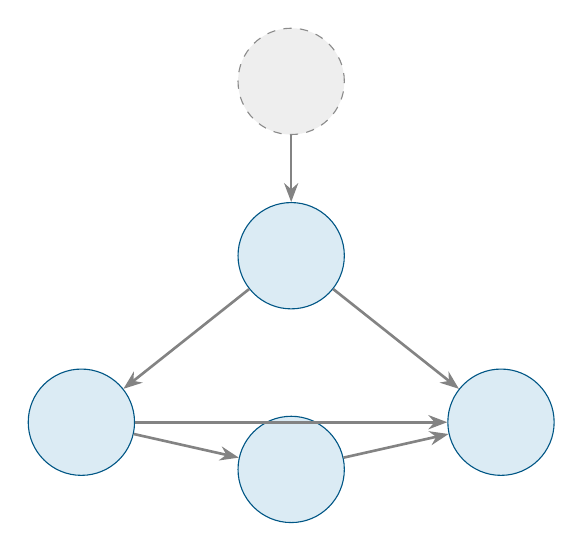
\begin{tikzpicture}[
  >={Stealth[length=2.4mm]},
  node distance=1.15cm and 1.7cm,
  obs/.style={
    circle, draw=otblue!75!black, fill=otblue!14,
    minimum size=1.35cm, align=center, font=\sffamily\footnotesize, inner sep=1pt,
  },
  unobs/.style={
    circle, draw=otgray!70, fill=otgray!10, dashed,
    minimum size=1.35cm, align=center, font=\sffamily\footnotesize, inner sep=1pt,
  },
  flow/.style={draw=otgray!75, line width=0.95pt, ->},
]
  \node[obs] (z) {\zlabel};
  \node[obs, below left=of z] (x) {\xlabel};
  \node[obs, below right=of z] (y) {\ylabel};
  \node[obs, below=1.35cm of z] (m) {\mlabel};
  \node[unobs, above=0.85cm of z] (u) {\ulabel};

  \draw[flow] (z) -- (x);
  \draw[flow] (z) -- (y);
  \draw[flow] (x) -- (m);
  \draw[flow] (m) -- (y);
  \draw[flow] (x) -- (y);
  \draw[flow] (u) -- (z);
\end{tikzpicture}
\end{document}
